\documentclass{anstrans}
%%%%%%%%%%%%%%%%%%%%%%%%%%%%%%%%%%%
\title{The Impact of Xenon-135 on Load Following Transatomic Power 
Molten Salt Reactor}

\author{Andrei Rykhlevskii, Daniel O'grady, Tomasz Kozlowski, Kathryn Huff}

\institute{
        Department of Nuclear, Plasma, and Radiological Engineering, University 
        of Illinois at Urbana-Champaign \break
        Urbana, IL
}

\email{andreir2@illinois.edu}

%%%% packages and definitions (optional)
\usepackage{graphicx} % allows inclusion of graphics
\usepackage{caption}  % allows center figures caption
\usepackage{booktabs} % nice rules (thick lines) for tables
\usepackage{microtype} % improves typography for PDF
\usepackage[section]{placeins}

\usepackage[acronym,toc]{glossaries}  % acronyms inclusion
%\newacronym{<++>}{<++>}{<++>}
\newacronym[longplural={metric tons of heavy metal}]{MTHM}{MTHM}{metric ton of heavy metal}
\newacronym{ABM}{ABM}{agent-based modeling}
\newacronym{ACDIS}{ACDIS}{Program in Arms Control \& Domestic and International Security}
\newacronym{AHTR}{AHTR}{Advanced High Temperature Reactor}
\newacronym{ANDRA}{ANDRA}{Agence Nationale pour la gestion des D\'echets RAdioactifs, the French National Agency for Radioactive Waste Management}
\newacronym{ANL}{ANL}{Argonne National Laboratory}
\newacronym{ANS}{ANS}{American Nuclear Society}
\newacronym{API}{API}{application programming interface}
\newacronym{ARE}{ARE}{Aircraft Reactor Experiment}
\newacronym{ARFC}{ARFC}{Advanced Reactors and Fuel Cycles}
\newacronym{ASME}{ASME}{American Society of Mechanical Engineers}
\newacronym{ATWS}{ATWS}{Anticipated Transient Without Scram}
\newacronym{BOL}{BOL}{Beginning of Life}
\newacronym{BDBE}{BDBE}{Beyond Design Basis Event}
\newacronym{BIDS}{BIDS}{Berkeley Institute for Data Science}
\newacronym{BWR}{BWR}{Boiling Water Reactor}
\newacronym{CAFCA}{CAFCA}{ Code for Advanced Fuel Cycles Assessment }
\newacronym{CDTN}{CDTN}{Centro de Desenvolvimento da Tecnologia Nuclear}
\newacronym{CFD}{CFD}{Computational Fluid Dynamics}
\newacronym{CEA}{CEA}{Commissariat \`a l'\'Energie Atomique et aux \'Energies Alternatives}
\newacronym{CI}{CI}{continuous integration}
\newacronym{CNEN}{CNEN}{Comiss\~{a}o Nacional de Energia Nuclear}
\newacronym{CNERG}{CNERG}{Computational Nuclear Engineering Research Group}
\newacronym{COSI}{COSI}{Commelini-Sicard}
\newacronym{COTS}{COTS}{commercial, off-the-shelf}
\newacronym{CSNF}{CSNF}{commercial spent nuclear fuel}
\newacronym{CTAH}{CTAHs}{Coiled Tube Air Heaters}
\newacronym{CUBIT}{CUBIT}{CUBIT Geometry and Mesh Generation Toolkit}
\newacronym{CURIE}{CURIE}{Centralized Used Fuel Resource for Information Exchange}
\newacronym{CR}{CR}{conversion ratio}
\newacronym{DAG}{DAG}{directed acyclic graph}
\newacronym{DANESS}{DANESS}{Dynamic Analysis of Nuclear Energy System Strategies}
\newacronym{DBE}{DBE}{Design Basis Event}
\newacronym{DESAE}{DESAE}{Dynamic Analysis of Nuclear Energy Systems Strategies}
\newacronym{DHS}{DHS}{Department of Homeland Security}
\newacronym{DOE}{DOE}{Department of Energy}
\newacronym{DRACS}{DRACS}{Direct Reactor Auxiliary Cooling System}
\newacronym{DRE}{DRE}{dynamic resource exchange}
\newacronym{DSNF}{DSNF}{DOE spent nuclear fuel}
\newacronym{DYMOND}{DYMOND}{Dynamic Model of Nuclear Development }
\newacronym{EBS}{EBS}{Engineered Barrier System}
\newacronym{EDF}{EDF}{Électricité de France}
\newacronym{EDZ}{EDZ}{Excavation Disturbed Zone}
\newacronym{EOL}{EOL}{End of Life}
\newacronym{EIA}{EIA}{U.S. Energy Information Administration}
\newacronym{EPA}{EPA}{Environmental Protection Agency}
\newacronym{EPR}{EPR}{European Pressurized Reactors}
\newacronym{EP}{EP}{Engineering Physics}
\newacronym{EU}{EU}{European Union}
\newacronym{FCO}{FCO}{Fuel Cycle Options}
\newacronym{FCT}{FCT}{Fuel Cycle Technology}
\newacronym{FEHM}{FEHM}{Finite Element Heat and Mass Transfer}
\newacronym{FEPs}{FEPs}{Features, Events, and Processes}
\newacronym{FHR}{FHR}{Fluoride-Salt-Cooled High-Temperature Reactor}
\newacronym{FLiBe}{FLiBe}{Fluoride-Lithium-Beryllium}
\newacronym{FP}{FP}{Fission Product}
\newacronym{GDSE}{GDSE}{Generic Disposal System Environment}
\newacronym{GDSM}{GDSM}{Generic Disposal System Model}
\newacronym{GENIUSv1}{GENIUSv1}{Global Evaluation of Nuclear Infrastructure Utilization Scenarios, Version 1}
\newacronym{GENIUSv2}{GENIUSv2}{Global Evaluation of Nuclear Infrastructure Utilization Scenarios, Version 2}
\newacronym{GENIUS}{GENIUS}{Global Evaluation of Nuclear Infrastructure Utilization Scenarios}
\newacronym{GPAM}{GPAM}{Generic Performance Assessment Model}
\newacronym{GRSAC}{GRSAC}{Graphite Reactor Severe Accident Code}
\newacronym{GUI}{GUI}{graphical user interface}
\newacronym{HLW}{HLW}{high level waste}
\newacronym{HPC}{HPC}{high-performance computing}
\newacronym{HTC}{HTC}{high-throughput computing}
\newacronym{HTGR}{HTGR}{High Temperature Gas-Cooled Reactor}
\newacronym{IAEA}{IAEA}{International Atomic Energy Agency}
\newacronym{IEMA}{IEMA}{Illinois Emergency Mangament Agency}
\newacronym{IHLRWM}{IHLRWM}{International High Level Radioactive Waste Management}
\newacronym{INL}{INL}{Idaho National Laboratory}
\newacronym{IPRR1}{IRP-R1}{Instituto de Pesquisas Radioativas Reator 1}
\newacronym{IRP}{IRP}{Integrated Research Project}
\newacronym{ISFSI}{ISFSI}{Independent Spent Fuel Storage Installation}
\newacronym{ISRG}{ISRG}{Independent Student Research Group}
\newacronym{JFNK}{JFNK}{Jacobian-Free Newton Krylov}
\newacronym{LANL}{LANL}{Los Alamos National Laboratory}
\newacronym{LBNL}{LBNL}{Lawrence Berkeley National Laboratory}
\newacronym{LCOE}{LCOE}{levelized cost of electricity}
\newacronym{LEU}{LEU}{low-enriched uranium}
\newacronym{LDRD}{LDRD}{laboratory directed research and development}
\newacronym{LFR}{LFR}{Lead-Cooled Fast Reactor}
\newacronym{LLNL}{LLNL}{Lawrence Livermore National Laboratory}
\newacronym{LMFBR}{LMFBR}{Liquid Metal Fast Breeder Reactor}
\newacronym{LOFC}{LOFC}{Loss of Forced Cooling}
\newacronym{LOHS}{LOHS}{Loss of Heat Sink}
\newacronym{LOLA}{LOLA}{Loss of Large Area}
\newacronym{LP}{LP}{linear program}
\newacronym{LWR}{LWR}{Light Water Reactor}
\newacronym{MAGNOX}{MAGNOX}{Magnesium Alloy Graphie Moderated Gas Cooled Uranium Oxide Reactor}
\newacronym{MA}{MA}{minor actinide}
\newacronym{MCNP}{MCNP}{Monte Carlo N-Particle code}
\newacronym{MILP}{MILP}{mixed-integer linear program}
\newacronym{MIT}{MIT}{the Massachusetts Institute of Technology}
\newacronym{MOAB}{MOAB}{Mesh-Oriented datABase}
\newacronym{MOOSE}{MOOSE}{Multiphysics Object-Oriented Simulation Environment}
\newacronym{MOSART}{MOSART}{Molten Salt Actinide Recycler and Transmuter}
\newacronym{MOX}{MOX}{mixed oxide}
\newacronym{MPI}{MPI}{Message Passing Interface}
\newacronym{MSBR}{MSBR}{Molten Salt Breeder Reactor}
\newacronym{MSFR}{MSFR}{Molten Salt Fast Reactor}
\newacronym{MSRE}{MSRE}{Molten Salt Reactor Experiment}
\newacronym{MSR}{MSR}{Molten Salt Reactor}
\newacronym{NAGRA}{NAGRA}{National Cooperative for the Disposal of Radioactive Waste}
\newacronym{NEAMS}{NEAMS}{Nuclear Engineering Advanced Modeling and Simulation}
\newacronym{NEUP}{NEUP}{Nuclear Energy University Programs}
\newacronym{NFCSim}{NFCSim}{Nuclear Fuel Cycle Simulator}
\newacronym{NGNP}{NGNP}{Next Generation Nuclear Plant}
\newacronym{NMWPC}{NMWPC}{Nuclear MW Per Capita}
\newacronym{NNSA}{NNSA}{National Nuclear Security Administration}
\newacronym{NPP}{NPP}{Nuclear Power Plant}
\newacronym{NPRE}{NPRE}{Department of Nuclear, Plasma, and Radiological Engineering}
\newacronym{NQA1}{NQA-1}{Nuclear Quality Assurance - 1}
\newacronym{NRC}{NRC}{Nuclear Regulatory Commission}
\newacronym{NSF}{NSF}{National Science Foundation}
\newacronym{NSSC}{NSSC}{Nuclear Science and Security Consortium}
\newacronym{NUWASTE}{NUWASTE}{Nuclear Waste Assessment System for Technical Evaluation}
\newacronym{NWF}{NWF}{Nuclear Waste Fund}
\newacronym{NWTRB}{NWTRB}{Nuclear Waste Technical Review Board}
\newacronym{OCRWM}{OCRWM}{Office of Civilian Radioactive Waste Management}
\newacronym{OOP}{OOP}{Object-Orienting Programming}
\newacronym{ORION}{ORION}{ORION}
\newacronym{ORNL}{ORNL}{Oak Ridge National Laboratory}
\newacronym{PARCS}{PARCS}{Purdue Advanced Reactor Core Simulator}
\newacronym{PBAHTR}{PB-AHTR}{Pebble Bed Advanced High Temperature Reactor}
\newacronym{PBFHR}{PB-FHR}{Pebble-Bed Fluoride-Salt-Cooled High-Temperature Reactor}
\newacronym{PEI}{PEI}{Peak Environmental Impact}
\newacronym{PH}{PRONGHORN}{PRONGHORN}
\newacronym{PRIS}{PRIS}{Power Reactor Information System}
\newacronym{PRKE}{PRKE}{Point Reactor Kinetics Equations}
\newacronym{PSPG}{PSPG}{Pressure-Stabilizing/Petrov-Galerkin}
\newacronym{PWAR}{PWAR}{Pratt and Whitney Aircraft Reactor}
\newacronym{PWR}{PWR}{Pressurized Water Reactor}
\newacronym{PyNE}{PyNE}{Python toolkit for Nuclear Engineering}
\newacronym{PyRK}{PyRK}{Python for Reactor Kinetics}
\newacronym{QA}{QA}{quality assurance}
\newacronym{RDD}{RD\&D}{Research Development and Demonstration}
\newacronym{RD}{R\&D}{Research and Development}
\newacronym{REE}{REE}{rare earth element}
\newacronym{RELAP}{RELAP}{Reactor Excursion and Leak Analysis Program}
\newacronym{RIA}{RIA}{Reactivity Insertion Accident}
\newacronym{RIF}{RIF}{Region-Institution-Facility}
\newacronym{SFR}{SFR}{Sodium-Cooled Fast Reactor}
\newacronym{SINDAG}{SINDA{\textbackslash}G}{Systems Improved Numerical Differencing Analyzer $\backslash$ Gaski}
\newacronym{SKB}{SKB}{Svensk K\"{a}rnbr\"{a}nslehantering AB}
\newacronym{SNF}{SNF}{spent nuclear fuel}
\newacronym{SNL}{SNL}{Sandia National Laboratory}
\newacronym{STC}{STC}{specific temperature change}
\newacronym{SUPG}{SUPG}{Streamline-Upwind/Petrov-Galerkin}
\newacronym{SVF}{SVF}{salt volume fraction}
\newacronym{SWF}{SWF}{Separations and Waste Forms}
\newacronym{SWU}{SWU}{Separative Work Unit}
\newacronym{TAP}{TAP}{Transatomic Power}
\newacronym{TRIGA}{TRIGA}{Training Research Isotope General Atomic}
\newacronym{TRISO}{TRISO}{Tristructural Isotropic}
\newacronym{TSM}{TSM}{Total System Model}
\newacronym{TSPA}{TSPA}{Total System Performance Assessment for the Yucca Mountain License Application}
\newacronym{ThOX}{ThOX}{thorium oxide}
\newacronym{UFD}{UFD}{Used Fuel Disposition}
\newacronym{UML}{UML}{Unified Modeling Language}
\newacronym{UOX}{UOX}{uranium oxide}
\newacronym{UQ}{UQ}{uncertainty quantification}
\newacronym{US}{US}{United States}
\newacronym{UW}{UW}{University of Wisconsin}
\newacronym{VISION}{VISION}{the Verifiable Fuel Cycle Simulation Model}
\newacronym{VVER}{VVER}{Voda-Vodyanoi Energetichesky Reaktor (Russian Pressurized Water Reactor)}
\newacronym{VV}{V\&V}{verification and validation}
\newacronym{WIPP}{WIPP}{Waste Isolation Pilot Plant}
\newacronym{YMR}{YMR}{Yucca Mountain Repository Site}

\usepackage{multirow} 
\usepackage{tabularx}
\newcolumntype{b}{>{\hsize=1.0\hsize}X}
\newcolumntype{s}{>{\hsize=.5\hsize}X}
\newcolumntype{m}{>{\hsize=.75\hsize}X}
\newcolumntype{x}{>{\hsize=.25\hsize}X}
\newcolumntype{a}{>{\hsize=.11\hsize}X}

\makeglossaries

\graphicspath{{figures/}}

\newcommand{\SN}{S$_N$}
\renewcommand{\vec}[1]{\bm{#1}} %vector is bold italic
\newcommand{\vd}{\bm{\cdot}} % slightly bold vector dot
\newcommand{\grad}{\vec{\nabla}} % gradient
\newcommand{\ud}{\mathop{}\!\mathrm{d}} % upright derivative symbol

\begin{document}
%%%%%%%%%%%%%%%%%%%%%%%%%%%%%%%%%%%%%%%%%%%%%%%%%%%%%%%%%%%%%%%%%%%%%%%%%%%%%%%%
\section{Introduction}
A First-of-its-kind civil \gls{MSR} was developed, built and operated in 
\gls{ORNL} in the 1960s. It was called the \gls{MSRE} and to this day, it is 
the only \gls{MSR} to have operated worldwide. Based on the experience 
from this experiment, the first commercial \gls{MSBR} was designed in early 
the 1970s. In a thermal spectrum \gls{MSR}, fluorides of fissile and/or 
fertile materials (i.e., UF$_4$ and/or ThF$_4$) are mixed with carrier salts 
(i.e., LiF) to form a liquid fuel, which is circulated in a loop-type primary 
circuit and leads to the following advantages over traditional solid-fueled 
reactors: (1) low pressure in the primary loop; (2) strong negative thermal 
feedback; (3) passive decay heat cooling; (4) reduced fuel fabrication costs; 
(5) online refueling and reprocessing \cite{haubenreich_experience_1970}.

Nevertheless, in order to be competitive in the current domestic energy 
market, these innovative designs may need the flexibility to follow load. 
Load following operation has the potential to increase the commercial 
competitiveness of nuclear power dramatically. Due to the increasing 
penetration of renewables into the electric grid, base-load operation carries 
the risk of correspondingly frequent negative electric energy pricing. Thus, 
responsiveness to the net electricity demand is essential to market relevance 
for new designs \cite{energy_information_administration_u.s._2016}.

The main physical effect that limits the possibilities of power variations in a 
conventional \gls{LWR} is fission product poisoning, especially the xenon 
effect (a few hours after the change in the reactor power level).  The 
$^{135}$Xe is the most powerful known neutron absorber (average cross section 
for thermal neutrons approximately $10^6$ barns) with a half-life  
$\tau_{1/2}=9.17h$ and yield for $^{235}$U fission about 6.3\%. The vast 
majority of xenon-135 (6.1\%) is produced from another fission product - 
$^{135}$I ($\tau_{1/2}=6.6h$) \cite{lokhov_technical_2011}. Under normal 
operating conditions, the $^{135}$Xe is being transmuted to $^{136}$Xe 
('burned') in the reactor core as it is produced, so while it harms the 
neutron economy, balancing the reactor controls can compensate 
for its effect. The difficulty comes when the reactor power is reduced, and 
there are fewer neutrons to burn out the $^{135}$Xe, so its concentration 
increases and further suppresses reactor power. In this case, the core takes 
some time to recover from the power reduction impact of $^{135}$Xe. This 
response to changing power levels, particularly from higher to lower power 
levels, dramatically slows the reactor's response to power demands. 
Potentially, $^{135}$Xe removal during reactor operation would allow more 
flexibly vary power levels to follow power demands, typically referred to 
as `load following.'

The \gls{TAP} \gls{MSR} design is a 1250 MW$_{th}$ liquid-fueled reactor which 
has been selected as a prototype of modern \gls{MSR}. The \gls{TAP} is an 
intermediate spectrum reactor designed to be started with high-assay \gls{LEU}
 as initial fissile load. This work presents modeling and simulation of 
load following transient operation of the \gls{TAP} \gls{MSR}. We 
compared these results with well-studied \gls{PWR} behavior. This study 
focuses on the $^{135}$Xe/$^{135}$I balance in the \gls{TAP} core and its 
effect on the reactor performance. Herein we assumed that the \gls{TAP} 
online fuel reprocessing system is inactive. Another feature of the \gls{MSR}, 
its circulating liquid fuel and corresponding delayed neutron precursor drift, 
is also not treated here.

Much of the analysis herein used a full-core 3-D model of the \gls{TAP} 
\gls{MSR} developed using the continuous-energy Serpent 2 Monte Carlo reactor 
physics software \cite{leppanen_serpent_2015}. The \gls{PWR} transient 
analysis has been done using the single-assembly model with burnable poison 
(gadolinium) provided with Serpent. All calculations presented in this paper 
were performed using the Serpent 2 version 2.1.31 with JEFF-3.1.2 nuclear data 
\cite{oecd/nea_jeff-3.1.2_2014}.
%%%%%%%%%%%%%%%%%%%%%%%%%%%%%%%%%%%%%%%%%%%%%%%%%%%%%%%%%%%%%%%%%%%%%%%%%%%%%%%%
\section{Description of the actual work}
\subsection{Transatomic Power Reactor Design}
The \gls{TAP} \gls{MSR} concept is very similar to original \gls{MSRE} design 
developed by \gls{ORNL} \cite{haubenreich_experience_1970} but it has two 
major innovations: 
the fuel salt composition and the moderator. The \gls{MSRE}'s  
LiF-BeF$_2$-ZrF$_4$-UF$_4$ salt has been substituted with LiF-UF$_4$ salt 
which allows for an increase in the uranium concentration within the fuel salt 
from 0.9 to 27.5\% while maintaining a relatively low melting point 
(490$^{\circ}$C compared with 434$^{\circ}$C for the original \gls{MSRE}'s 
salt) \cite{betzler_assessment_2017}. The graphite has a very high 
thermal scattering cross section which makes it a perfect moderator but it has 
a few major drawbacks: 
(1) the low lethargy gain per collision requires a large volume of moderator 
to be present to reach criticality, which leads to a larger core and obstructs 
the core power density; (2) even special 
reactor-grade graphite has relatively high porosity, consequently, it holds
gaseous \glspl{FP} 
(e.g., tritium, xenon) in pores; (3) the reactor graphite lifespan in a 
commercial 
reactor is about 10 years \cite{robertson_conceptual_1971}. To resolve these 
issues, the \gls{TAP} concept uses another 
moderator, namely, zirconium hydride (ZrH$_{1.66}$), allowing for a more 
compact core and a 
significant increase in power density. These two innovative design choices,  
together with a configurable moderator 
(the moderator-to-fuel ratio can be changed during regular maintenance 
shutdown), 
facilitate the commercial deployment of this conceptual design in the current 
commercially available 5\% \gls{LEU} fuel cycle. 

The \gls{TAP} \gls{MSR} primary loop contains the reactor core volume 
(including the zirconium hydride moderator rods with silicone carbide 
cladding), pumps, and primary heat exchanger. Pumps circulate the 
LiF-(Act)F$_4$ fuel salt through the primary loop. The pumps, vessels, tanks, 
and piping are made of a nickel-based alloy (similar to Hastelloy-N\footnote{ 
Hastelloy-N  is very common in reactors now and have been studied and 
developed at \gls{ORNL} in a program that started in the 1950s.}), which is 
highly resistant to corrosion in various molten salt environments. Inside the 
reactor vessel, near the zirconium hydride moderator rods, 
the fuel salt is in a critical configuration and generates heat. 
Table~\ref{tab:tap_tab} contains details of the \gls{TAP} system design. 
%%%%%%%%%%%%%%%%%%%%%%%%%%%%%%%%%%%%%%%%
\begin{table}[h!]
	\caption{Summary of principal data for the \gls{TAP} \gls{MSR} 	
	\cite{transatomic_power_corporation_technical_2016, 
	transatomic_power_corporation_neutronics_2016}). }
	\begin{tabularx}{\linewidth}{X  X }
		\hline
		Thermal power		& 1250 MW$_{th}  $       
		\\ 
		Electric power		& 520 MW$_e  $ 			 
		\\ 
		Gross thermal efficiency 	& 44\%     				 
		\\  
		Outlet temperature			& 620$^{\circ}$C         
		\\ 
		Fuel salt components        & LiF-UF$_4$				 \\  
		Fuel salt composition       & 72.5-27.5 mole\%			 
		\\  
		Uranium enrichment          & 5\% $^{235}$U          	 \\
		Moderator & Zirconium Hydride (ZrH) with SiC 
		cladding \\
		Neutron spectrum						& 
		thermal/epithermal                 \\
		\hline
	\end{tabularx}
	\label{tab:tap_tab}
\end{table}
\subsection{TAP Full-core Model} \label{sec:tap_model}
The advanced geometry surface and transformation capabilities of Serpent are 
employed to represent the \gls{TAP} core. Fig.~\ref{fig:tap-serpent-plan} shows 
the $XY$ section of whole-core configuration at the expected reactor 
operational level when all control rods are fully withdrawn. This model 
contains the moderator rods with silicon carbide cladding, pressure vessel, 
inlet and outlet plena (Table~\ref{tab:tap_model_param}). Fuel salt flows 
through rectangular moderator assemblies consisting of lattices of 
small-diameter zirconium hydride rods in a corrosion-resistant material. 
Moderator rods configuration is selected to obtain \gls{SVF}  
($SVF=V_{fuel}/(V_{fuel}+V_{moder})$) approximately 0.9 
\cite{betzler_assessment_2017}.
%%%%%%%%%%%%%%%%%%%%%%%%%%%%%%%%%%%%%%%%%%%%%%%%%%
\begin{table}[h!]
	\caption{Geometric parameters for the full-core 3D model of 
		the \gls{TAP} \cite{betzler_assessment_2017}. }
	\centering
	\begin{tabularx}{\linewidth}{s s x p{0.12\linewidth}}
		\hline
		\textbf{Component} & \textbf{Parameter} & Value      		& 
		Unit		             \\ \hline
		\multirow{4}{*}{\begin{tabular}[c]{@{}l@{}}Moderator\\ 
				rod\end{tabular}} 
		& Cladding thickness      	  			    & 0.10 & cm				 
		\\  
		& Radius 				      	  			& 1.15 & cm				 
		\\  
		& Length				      	  			& 3.0  & m				 
		\\  
		& Pitch				      	  			& 3.0  & cm  			 \\ 
		\hline 
		
		\multirow{2}{*}{\begin{tabular}[c]{@{}l@{}}Moderator\\ 
				assembly\end{tabular}} 
		& Array				      	  			& 5 $\times$ 5 & 
		rods$\times$rods \\  
		& Pitch				      	  			& 15.0 & cm    				 
		\\  \hline
		
		\multirow{4}{*}{\begin{tabular}[c]{@{}l@{}}Core\end{tabular}}          
		& Assemblies  				   	  			& 268  & pcs/core 
		\\  
		& Inner radius			      	  			& 1.5  & 
		m    				 \\  
		& Plenum height			   	  			& 25.0 & cm    				 
		\\  
		& Vessel wall thickness     	  			& 5.0 & 
		cm    				 \\ \hline            
	\end{tabularx}
	\label{tab:tap_model_param}
\end{table}
%%%%%%%%%%%%%%%%%%%%%%%%%%%%%%%%%%%%%%%%%%%%%%%%
\begin{figure}[htp!] % replace 't' with 'b' to 
	\centering
	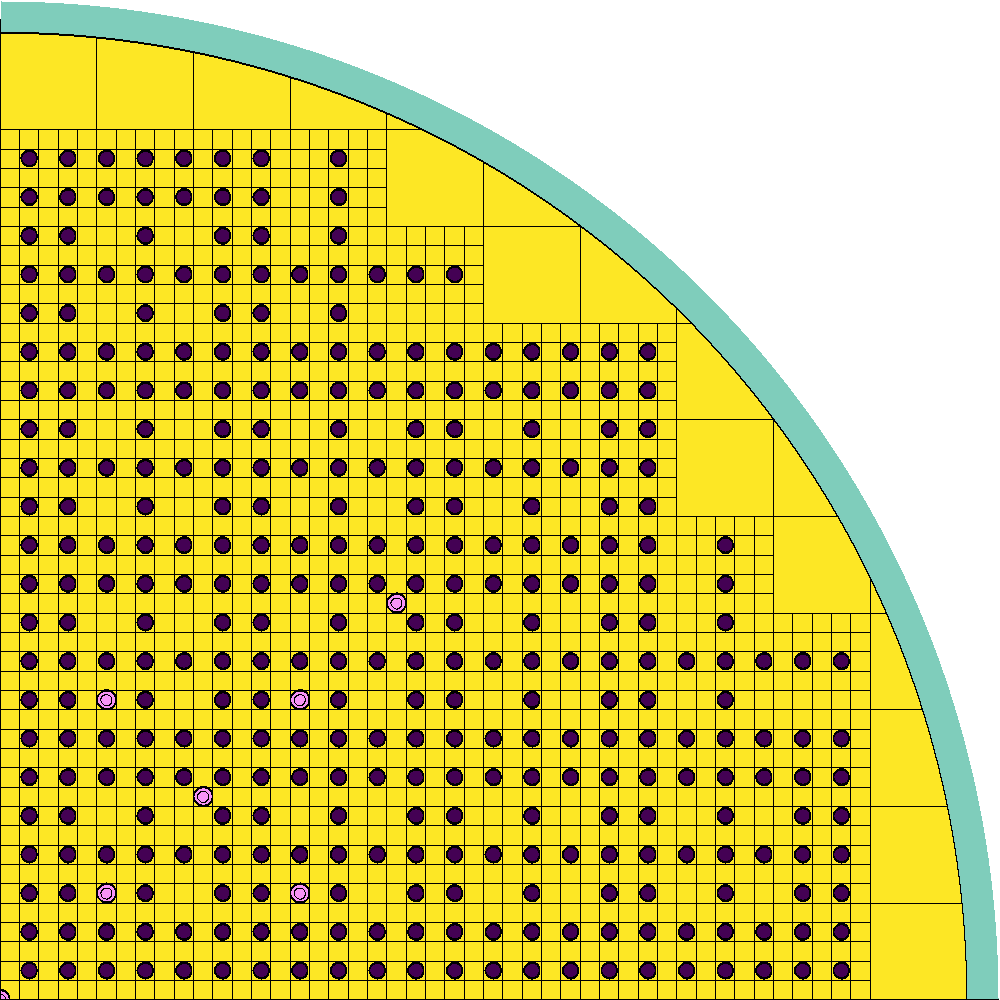
\includegraphics[width=\linewidth]{tap_plan_view.png}
	\caption{An $XY$ section of the \gls{TAP} model at the horizontal midplane 
		with fully withdrawn control rods. The violet color represents 
		zirconium hydride, and the yellow represents fuel salt. The blue color 
		shows Hastelloy-N, a material used for the vessel wall, and the pink 
		color is the air.}
	\label{fig:tap-serpent-plan}
\end{figure}

To represent the reactivity control system the 
model has: (1) control rod guide tubes made of a nickel-based alloy; (2) 
control 
rods represented as hollow 70-30\% Gd$_2$O$_3$-Al$_2$O$_3$ cylinders with a 
thin Hastelloy-N coating \cite{betzler_assessment_2017}; (3) air inside guide 
tube and control rod. Control rods design has yielded a cluster of 25 rods 
that provide a total reactivity worth of $1121\pm26$ pcm\footnote{ 1 pcm = 
10$^{-5}\Delta k_{eff}/k_{eff}$.}.
\subsection{Load Following Transient}
A generic \gls{PWR} during steady-state operation at a constant neutron flux 
level reaches $^{135}$Xe/$^{135}$I equilibrium for that reactor power in about 
40 to 60 hours. When the power level is decreased, the neutron flux is 
reduced, less $^{135}$Xe is transmuted ('burned') to $^{136}$Xe, and the 
balance shifts to the larger $^{135}$Xe concentration. In the worst-case 
scenario for the \gls{PWR} (power was reduced to 0\%) the xenon concentration 
peaks in about 8-9 hours following a shutdown (depending on the neutron 
spectrum). Based on this knowledge of \gls{PWR} poisoning, we selected 
following worst-case load curve (see figure~\ref{fig:pwr_keff}, 
\ref{fig:tap_keff}; red line):
\begin{enumerate}
	\item Startup with fresh fuel and operating on 
	100\% power level for 96 hours to reach $^{135}$Xe/$^{135}$I balance;
	\item Instantaneous variation of the power from 100\% to 0\%;
	\item Shutdown for 7.66 hours to reach the $^{135}$Xe peak;
	\item Instantaneous power boost from 0\% to 100\%, then operation on 
	this level for 16 hours.
\end{enumerate}
This scenario can be considered as backing up solar power with nuclear on a 
high-solar penetration grid (e.g., in California).

\section{Results and Analysis}
Using the methodology described previously, the \gls{PWR} assembly and 
the \gls{TAP} full core depletion analysis was performed. 
We used 15-min power load curve resolution during the active phase of the 
transient to capture rapid changes in multiplication factor and isotopic 
composition. All results herein were obtained using built-in Serpent 2 
capabilities for fuel depletion calculations.

\subsection{Multiplication Factor and Xenon Equilibrium}
Fig.~\ref{fig:pwr_keff} shows the infinite multiplication factor 
($k_{\infty}$) evolution for the \gls{PWR} assembly during postulated 
transient. As expected, $k_{\infty}$ dropped  after shutdown from 1.120 to 
1.105 ($-1500$ pcm) because $^{135}$I decayed to $^{135}$Xe, and xenon 
poisoned the core. The multiplication factor reached local minimum  
$\approx7$ hours after shutdown. Notably, after power level growth from 
0\% back to 100\%, 
$k_{\infty}$ reached even larger value than it was before shutdown ($\approx 
1.1234$, $+300$ pcm). The imbalance between $^{135}$I production and 
$^{135}$Xe 'burning' is a main reason of this reactivity boost.
\begin{figure}[htbp!] % replace 't' with 'b' to force it to be on the bottom
	\centering
	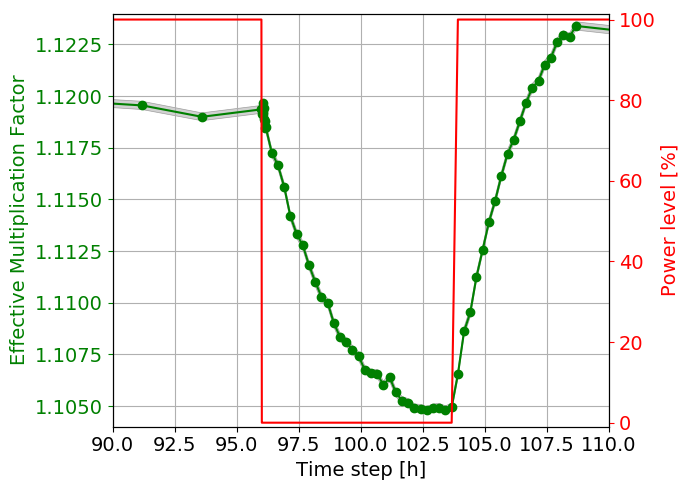
\includegraphics[width=1.03\linewidth]{pwr_keff_zoomed.png}
		\vspace{-0.25in}
	\caption{Multiplication factor for worst-case load curve for the \gls{PWR} 
	immediately after shutdown (confidence interval $\sigma\pm20$pcm shaded).}
		\vspace{-0.05in}
	\label{fig:pwr_keff}
\end{figure}

Fig.~\ref{fig:tap_keff} demonstrates the effective multiplication factor 
($k_{eff}$) dynamics in the same transient for full-core \gls{TAP} \gls{MSR} 
model without any online \gls{FP} removal. Surprisingly, $k_{eff}$ slowly 
increased after shutdown from 1.0065 to 1.0078 ($+130$ pcm), and overall  
reactivity swing for the scenario is much smaller (270 pcm difference between 
maximum and minimum vs. 1750 pcm for the \gls{PWR}). Similarly to the \gls{PWR} 
case, $k_{eff}$ for the \gls{TAP} jumped after reactor power turned back to 
100\% but by 150 pcm only. 
\begin{figure}[htbp!] % replace 't' with 'b' to force it to be on the bottom
	\centering
	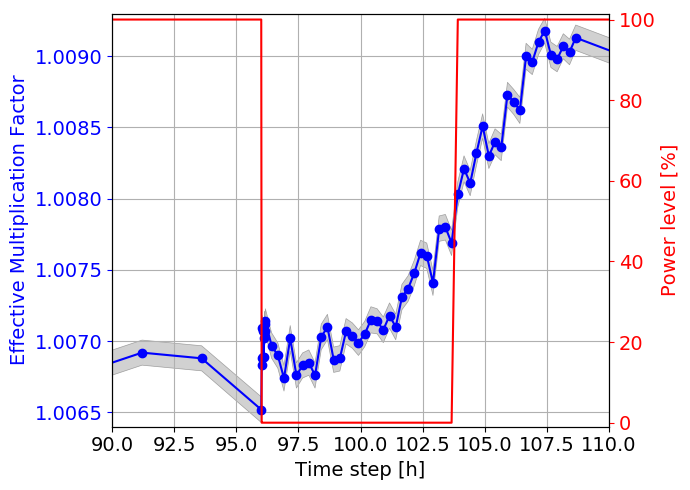
\includegraphics[width=1.03\linewidth]{tap_keff_zoomed.png}
		\vspace{-0.25in}
	\caption{Multiplication factor for worst-case load curve for the \gls{TAP} 
	immediately after shutdown ($\sigma\pm7.5$pcm shaded).}
		\vspace{-0.05in}
	\label{fig:tap_keff}
\end{figure}

The analysis of the fuel composition variation gives clearer information about 
the $^{135}$Xe/$^{135}$I equilibrium and the core state. Fig.~\ref{fig:compos} 
shows the number density of isotopes influential to core neutronics. After 96 
hours of operation on 100\% power level xenon reached 
equilibrium concentration, and $^{135}$I/$^{135}$Xe number density ratio is 
2.3 and 0.9 for the \gls{PWR} and \gls{TAP}, respectively. After shutdown the 
$^{135}$I decays to $^{135}$Xe that is not burned up. The \gls{PWR} had large 
$^{135}$I inventory which caused notable xenon concentration peak by 150\% 
from equilibrium after about 7 hours due to shorter $^{135}$I half-life (6.6h 
vs. 9.17h for $^{135}$Xe). Contrarily, in the \gls{TAP} $^{135}$Xe 
concentration remained unchanged after shutdown because $^{135}$I inventory 
was lower than $^{135}$Xe. Thus, $^{135}$Xe gain from $^{135}$I decay did not 
overcome $^{135}$Xe decay loss. In sum, the poisoning effect does not impact  
on the \gls{TAP} core reactivity even in worst-case transient due to 
much lower than in the \gls{PWR} $^{135}$I/$^{135}$Xe ratio at equilibrium.
\begin{figure}[htbp!] % replace 't' with 'b' to force it to be on the bottom
        \centering
        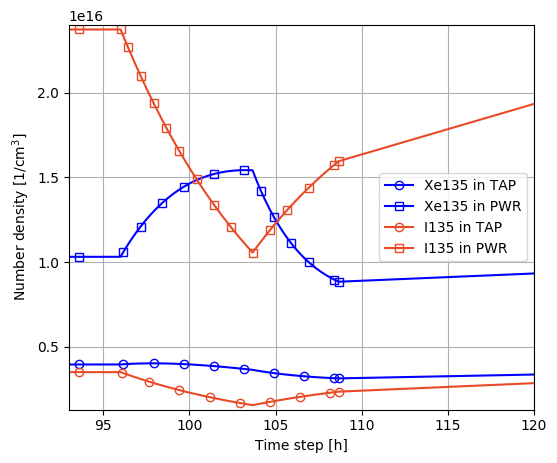
\includegraphics[width=1.07\linewidth]{tap_vs_pwr_xe_i_density.png}
        \caption{Atomic density of $^{135}$Xe and its precursor ($^{135}$I) 
        immediately after shutdown for the \gls{TAP} and \gls{PWR}.}
        \vspace{-0.2in}
        \label{fig:compos}
\end{figure}

\subsection{Neutron spectrum}
To understand the  difference between $^{135}$I/$^{135}$Xe gain and loss for 
two reactor types, we plotted the neutron flux per lethargy energy 
distribution (fig.~\ref{fig:spectrum}). The spectrum for the \gls{TAP} is 
harder than for the \gls{PWR} due to lack of moderation in the \gls{TAP} core 
(\gls{SVF}$\approx0.9$) and its type (ZrH). The harder neutron spectrum leads 
to weaker $^{135}$Xe transmutation because capture cross section is declined 
rapidly with energy (fig.~\ref{fig:spectrum}, solid red line, energy interval 
from $10^{-7}$ to $10^{-4}$). As a result, the \gls{TAP} \gls{MSR} $^{135}$Xe 
concentration surpasses the $^{135}$I concentration, shown in 
Fig.~\ref{fig:tap_keff}, preventing an excessive build up of $^{135}$Xe during 
transients.
\begin{figure}[htbp!] % replace 't' with 'b' to force it to be on the bottom
        \centering
        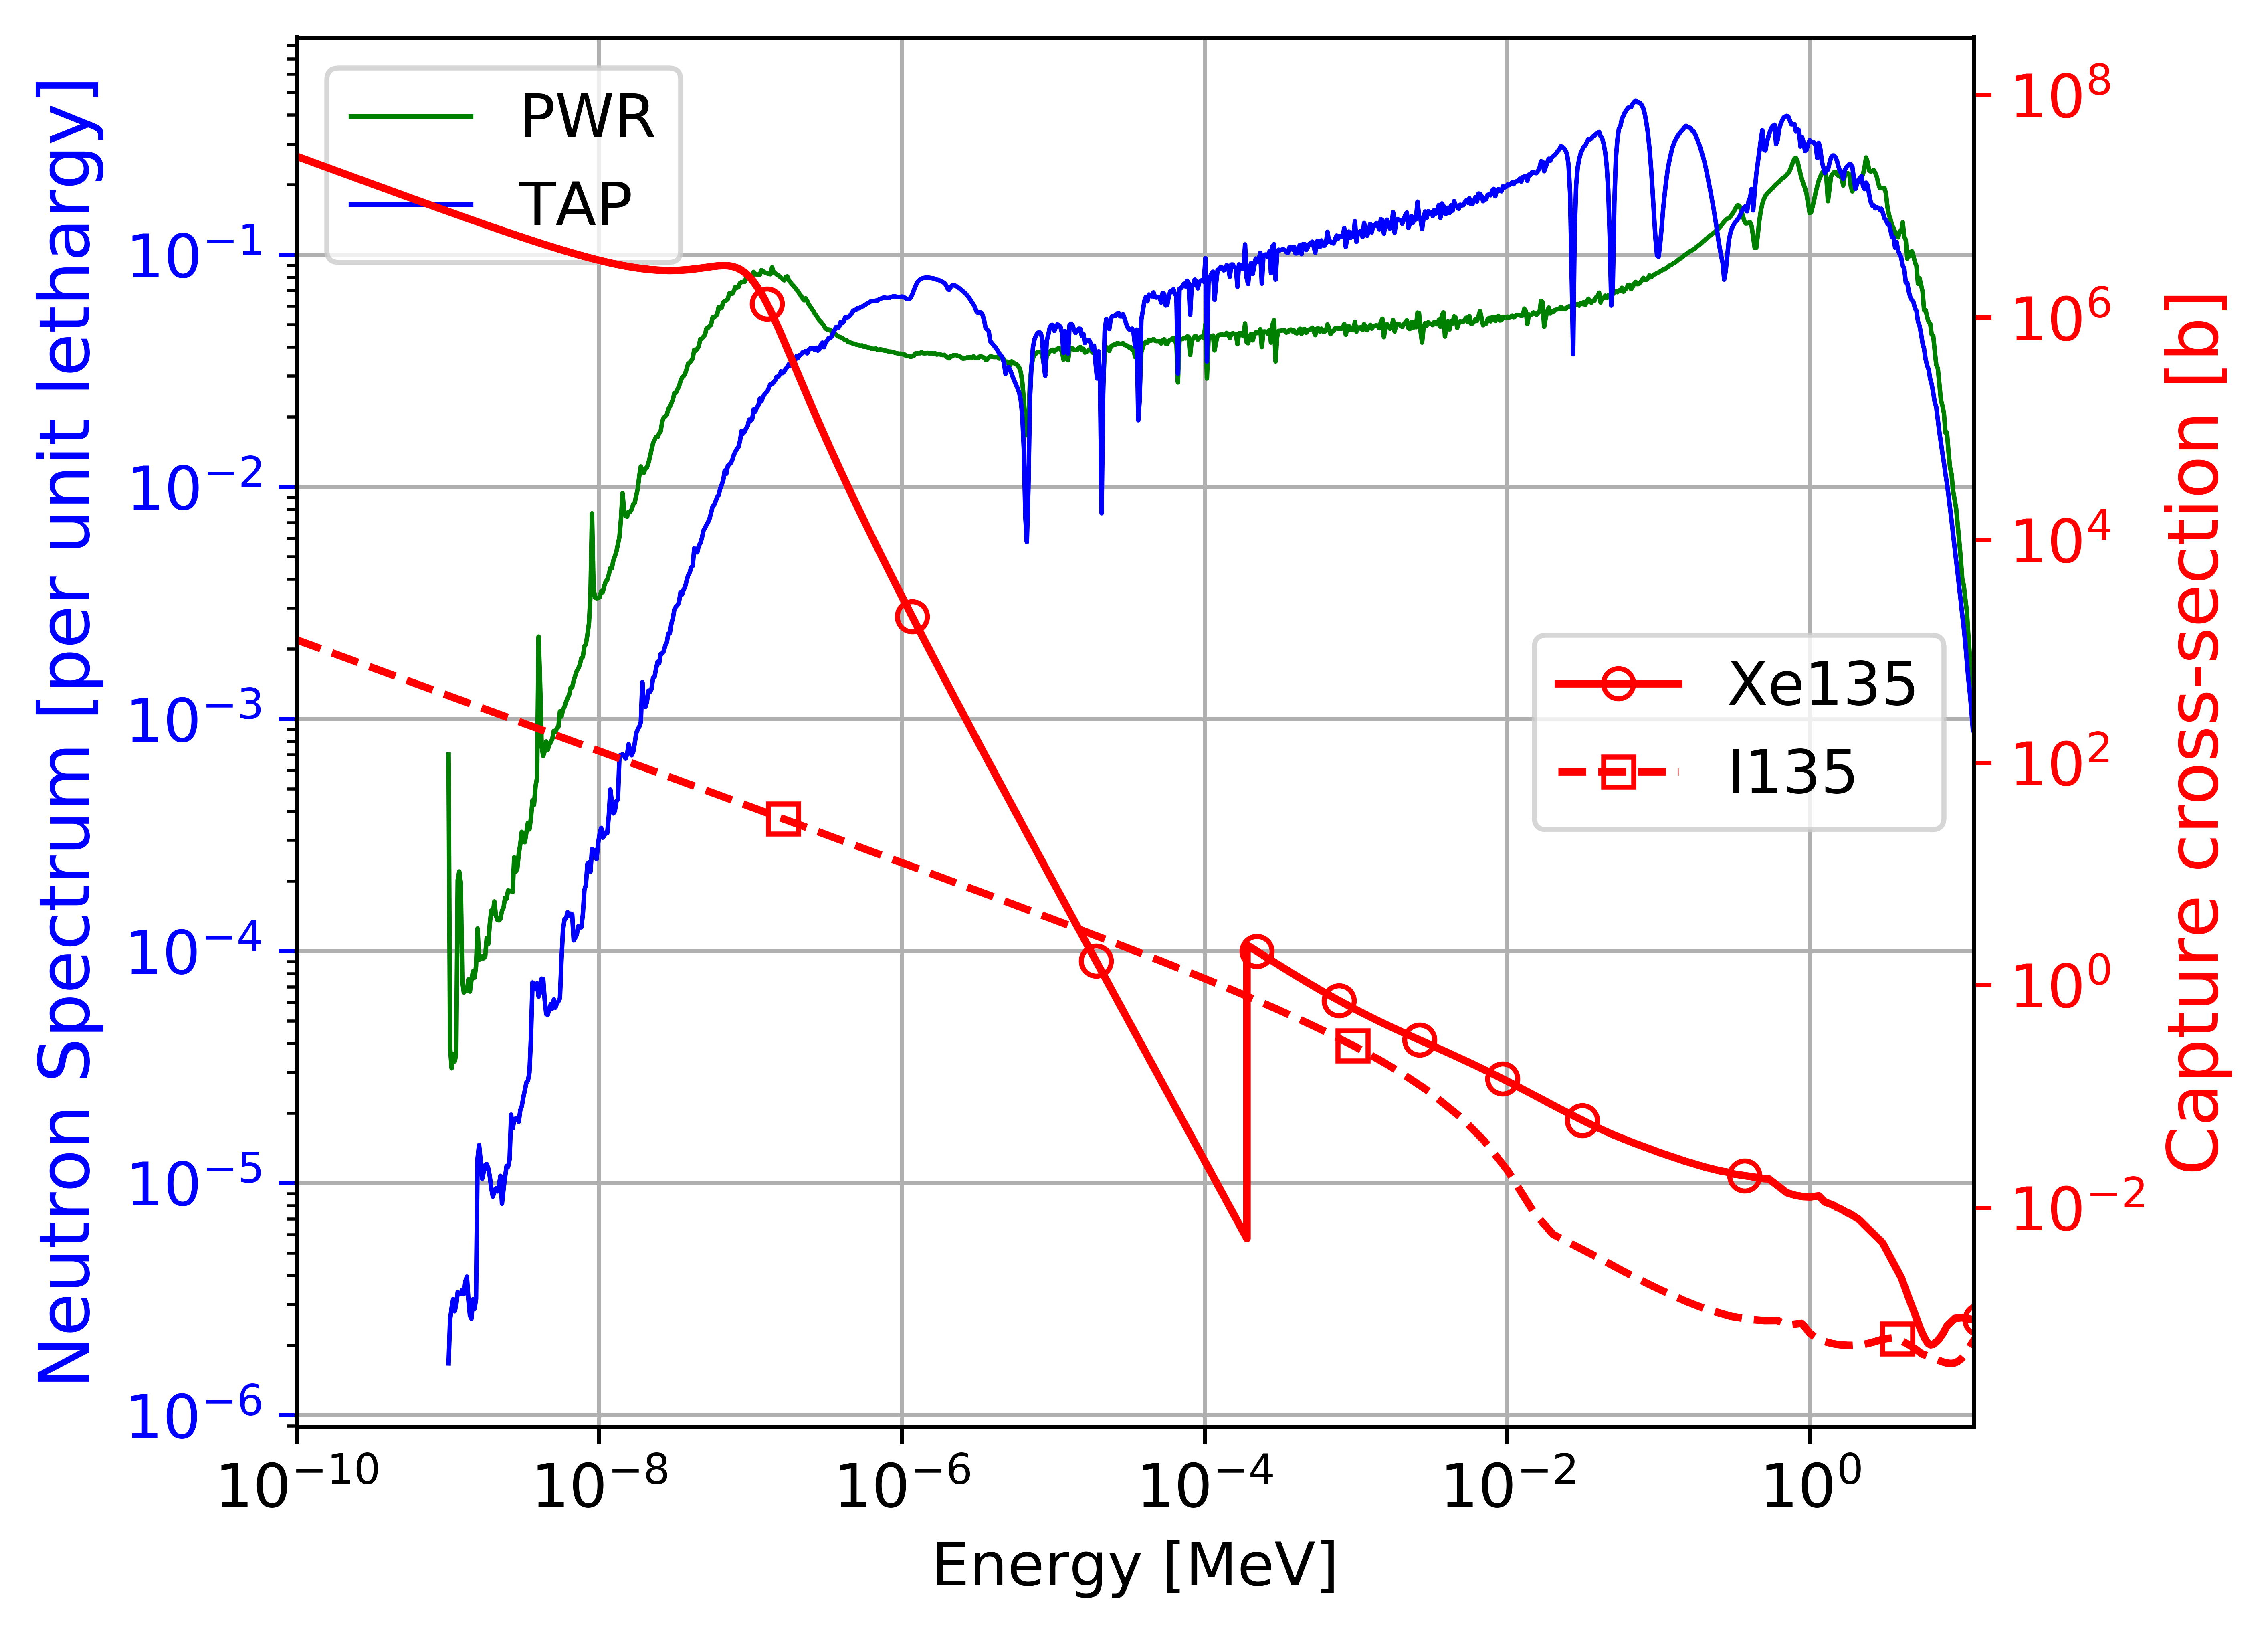
\includegraphics[width=1.07\linewidth]{spectra.png}
	        \vspace{-0.2in}
        \caption{Neutron spectra normalized by lethargy for the \gls{PWR} and 
        \gls{TAP} vs. $^{135}$Xe and $^{135}$I 
        caption cross-section.}
        	\vspace{-0.19in}
        \label{fig:spectrum}
\end{figure}
%%%%%%%%%%%%%%%%%%%%%%%%%%%%%%%%%%%%%%%%%%%%%%%%%%%%%%%%%%%%%%%%%%%%%%%%%%%%%%%%
\section{Conclusions}
The depletion calculations of the \gls{PWR} assembly and the \gls{TAP} 
full-core models for simple load following transient were performed using the 
Serpent 2 Monte Carlo code to illuminate the impact of Xenon-135 poisoning on 
the \gls{MSR}. The transient assumed for both reactor types following 
generated power dynamics: 
(1) 96-hour operation cycle on 100\% power level; (2) instant power drop to 
0\% level for 7.66 hours (to reach $^{135}$Xe concentration peak); (3) boost 
back to 100\% power, and operation on this level for 16 hours. The results of 
this study indicate that from the depletion calculation, the multiplication 
factor for the \gls{PWR} dropped rapidly after reactor shutdown and reached 
maximum poisoning effect (-1500pcm) $\approx7$ hours after shutdown. The drop  
happened because $^{135}$I/$^{135}$Xe number density ratio at equilibrium in 
the \gls{PWR} is about 2.3 and $^{135}$I decays to $^{135}$Xe faster than 
$^{135}$Xe to $^{135}$Cs.

Similar depletion calculation for the \gls{TAP} \gls{MSR} showed different 
result: $k_{eff}$ rose a bit after the reactor shutdown, and no effect of xenon 
poisoning was observed. The reason for this behavior is different 
$^{135}$I/$^{135}$Xe concentration ratio which is about 0.9. Thus, $^{135}$I 
decay did not lead to the xenon peak in the \gls{TAP} and the poisoning effect 
is negligible. The most obvious finding to emerge from the analysis is that the 
neutron energy spectrum is harder for the \gls{TAP}. The reactor neutron energy
spectrum significantly impacts $^{135}$Xe 'burn' rate and shifts  
$^{135}$I/$^{135}$Xe mass balance at equilibrium.

Continued research into the \gls{MSR} load following and related topics 
could progress in many different directions. First and foremost, efforts will 
be made to investigate the impact of xenon poisoning on \gls{TAP} in the 
end-of-life (EOL) state, which might have a more thermal neutron spectrum. 
This 
might be performed with the online reprocessing tool SaltProc 
\cite{rykhlevskii_modeling_2019,rykhlevskii_arfc/saltproc:_2018}, which would  
simulate online fuel reprocessing and refueling to obtain realistic 
equilibrium fuel salt composition. Furthermore, the \gls{TAP} design allows 
the moderator-to-fuel ratio adjustment during operation, which should be taken 
into consideration in future simulations.

Lastly, an additional area to explore is the multi-physics transient analysis, 
which requires the development of the \gls{TAP} model with the coupled 
neutronics/thermal-hydraulics code, Moltres \cite{lindsay_introduction_2018}. 
The final goal of this effort is to characterize neutronics, and 
thermal-hydraulics limits related to load following, and optimize control rod 
maneuver strategy that minimizes axial offset and maintains safety margins.

\section{Acknowledgments}
This research was supported by the DOE ARPA-E MEITNER program award 
DE-AR0000983.
%%%%%%%%%%%%%%%%%%%%%%%%%%%%%%%%%%%%%%%%%%%%%%%%%%%%%%%%%%%%%%%%%%%%%%%%%%%%%%%%
\bibliographystyle{ans}
\bibliography{2019-rykhl-xenon-ans}
\end{document}

